\subsection{Investigation}
Students were first instructed to explore the provided circuit and become familiar with the appropriate pin locations.  This was accomplished by testing the values of~$V_\text{CC}$~(measured at~\SI{5.03}{\volt}) and~$V_\text{REF}$~(measured to be~\SI{2.509}{\volt}) to ensure that they were within reasonable limits of the expected values.  Once this was accomplished, the frequency and peak-to-peak voltage of the ADC's clock signal were measured to be~\SI{370.4}{\kilo\hertz} and~\SI{4.75}{\volt}, respectively.  This clock signal can be seen in the oscilloscope screenshot in Figure~\ref{fig:normalClock}.
%
\begin{figure}[H]
	\centering
	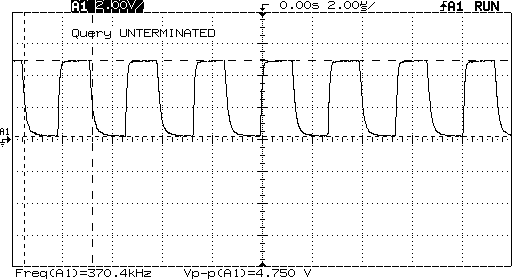
\includegraphics[width=.6\textwidth]{img/shot/part2shot.png}
	\parbox{.6\textwidth}{
	\caption[Typical ADC clock signal]{Oscilloscope of a typical clock signal
	for the ADC circuit.  No additional components were added here.}
	\label{fig:normalClock}}
\end{figure}
%
The lab instructions provide that the peak-to-peak voltage should be roughly~\SI{5}{\volt}, implying that the measured value is~\SI{5}{\percent} lower than designed. The instructions also state that the clock frequency can be calculated via~\eqref{eq:clock}:
%
\begin{equation}
	f_\text{CLK} = \frac{1}{2 R_T C_3} \label{eq:clock}
\end{equation}
%
where~$R_T$ is equal to the value of~$R_1$ for the schematic in Figure~\ref{fig:adcSchem} and~$C_3$ is as shown in the schematic, or~\SI{10}{\kilo\ohm} and~\SI{150}{\pico\farad} respectively.  These values equate to a theoretical clock frequency of~\SI{333.333}{\kilo\hertz}, meaning that the measured value is~\SI{11}{\percent} higher than the theoretical.  As it requires~70 clock pulses to complete the analog-to-digital conversion for one sample, this implies an experimental sampling frequency~$f_s$ of~\SI{5.29}{\kilo\hertz}~--- a difference of~\SI{12.5}{\percent} over the~\SI{4.7}{\kilo\hertz} frequency for which the system was designed.  This will actually make the system more accurate however, as was previously discussed.
%
Next, students placed another~\SI{10}{\kilo\ohm} resistor in parallel with~$R_1$ to monitor the effects of a halved resistance.  This resulted in the clock signal shown in Figure~\ref{fig:fastClock}.
%
\begin{figure}[H]
	\centering
	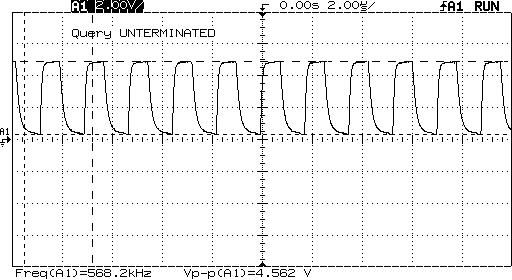
\includegraphics[width=.6\textwidth]{img/shot/part2bshot.png}
	\parbox{.6\textwidth}{
	\caption[Atypical ADC clock signal]{Measured clock signal after placing an additional~\SI{10}{\kilo\ohm} resistor across~$R_1$, thus halving the equivalent resistance.  Note that this had a profound effect on the signal's frequency compared to Figure~\ref{fig:normalClock} but a minor effect on its peak-to-peak voltage.}
	\label{fig:fastClock}}
\end{figure}
%
As can be seen by comparing the screenshots, the frequency increased by~\SI{53}{\percent} to~\SI{568.2}{\kilo\hertz}, while the peak-to-peak voltage decreased~\SI{4}{\percent} to~\SI{4.562}{\volt}.  This increased frequency is actually below its theoretical value by~\SI{15}{\percent}, as~\eqref{eq:clock} states that the frequency should have actually doubled to~\SI{666.666}{\kilo\hertz} with a halved resistance~$R_1$.  Once this measurement was made, the extra resistor was removed to restore the system back to its proper state.

\subsection{Zero Input}
To ensure that the converter was powered correctly, students shorted the input at pin~6 to ground to ensure that there was zero input voltage.  This should produce a binary output value of~\texttt{0000~0000}, resulting in all eight LEDs being turned on.  Once this happened, the short between~$V_\text{in}+$ and ground was removed.

\subsection{DC Input}
At this point in the experiment students were properly prepared to begin testing the ADC.  Using the in-lab DC power supply, the input voltage at pin~6 was varied from zero to five volts in one-volt increments, recording the output of the LEDs (and the associated binary representation) at each step.  These results can be seen in Figure~\ref{fig:pt4bars}.
%
\begin{figure}[H]
	\centering
	\begin{tikzpicture}[node distance=.5cm, auto, >=latex']
   \tikzstyle{off}=[rectangle, draw, minimum width=4em, minimum height=1em]
   \tikzstyle{on} =[rectangle, draw=red, fill=red, minimum width=4em, minimum height=1em]

   % bar one
   \begin{scope}
   	% outer box
   	\draw (-2.5em,1em) rectangle (2.5em,-11em);

   	% labels -- ONLY DO THESE ONCE
   	\draw (-2.5em, 1em) node[left] {LSB};
   	\draw (-2.5em,-11em) node[left] {MSB};

   	% led bars
   	\node[on] (bit0) {};
   	\node[on,  below of=bit0] (bit1) {};
   	\node[on,  below of=bit1] (bit2) {};
   	\node[on, below of=bit2] (bit3) {};

   	\node[on, below of=bit3] (bit4) {};
   	\node[on, below of=bit4] (bit5) {};
   	\node[on, below of=bit5] (bit6) {};
   	\node[on,  below of=bit6] (bit7) {};

   	% voltage
   	\node[below of=bit7, yshift=-.5em] (voltage) {\SI{0}{\volt}};

   	% bit mask
   	\node[below of=voltage] (bitMask) {\texttt{0000 0000}};
   \end{scope}

   \begin{scope}[xshift = 2.5cm]
   	% outer box
   	\draw (-2.5em,1em) rectangle (2.5em,-11em);

   	% led bars
   	\node[off] (bit0) {};
   	\node[off, below of=bit0] (bit1) {};
   	\node[on,  below of=bit1] (bit2) {};
   	\node[on,  below of=bit2] (bit3) {};

   	\node[off, below of=bit3] (bit4) {};
   	\node[off, below of=bit4] (bit5) {};
   	\node[on,  below of=bit5] (bit6) {};
   	\node[on,  below of=bit6] (bit7) {};

   	% voltage
   	\node[below of=bit7, yshift=-.5em] (voltage) {\SI{1}{\volt}};

   	% bit mask
   	\node[below of=voltage] (bitMask) {\texttt{0011 0011}};
   \end{scope}

   \begin{scope}[xshift = 5cm]
   	% outer box
   	\draw (-2.5em,1em) rectangle (2.5em,-11em);

   	% led bars
   	\node[on] (bit0) {};
   	\node[off, below of=bit0] (bit1) {};
   	\node[off, below of=bit1] (bit2) {};
   	\node[on,  below of=bit2] (bit3) {};

   	\node[on,  below of=bit3] (bit4) {};
   	\node[off, below of=bit4] (bit5) {};
   	\node[off, below of=bit5] (bit6) {};
   	\node[on,  below of=bit6] (bit7) {};

   	% voltage
   	\node[below of=bit7, yshift=-.5em] (voltage) {\SI{2}{\volt}};

   	% bit mask
   	\node[below of=voltage] (bitMask) {\texttt{0110 0110}};
   \end{scope}

   \begin{scope}[xshift = 7.5cm]
   	% outer box
   	\draw (-2.5em,1em) rectangle (2.5em,-11em);

   	% led bars
   	\node[on] (bit0) {};
   	\node[on,  below of=bit0] (bit1) {};
   	\node[off, below of=bit1] (bit2) {};
   	\node[off, below of=bit2] (bit3) {};

   	\node[off, below of=bit3] (bit4) {};
   	\node[off, below of=bit4] (bit5) {};
   	\node[on,  below of=bit5] (bit6) {};
   	\node[on,  below of=bit6] (bit7) {};

   	% voltage
   	\node[below of=bit7, yshift=-.5em] (voltage) {\SI{3}{\volt}};

   	% bit mask
   	\node[below of=voltage] (bitMask) {\texttt{0011 1100}};
   \end{scope}

   \begin{scope}[xshift = 10cm]
   	% outer box
   	\draw (-2.5em,1em) rectangle (2.5em,-11em);

   	% led bars
   	\node[on] (bit0) {};
   	\node[on,  below of=bit0] (bit1) {};
   	\node[off, below of=bit1] (bit2) {};
   	\node[off, below of=bit2] (bit3) {};

   	\node[on,  below of=bit3] (bit4) {};
   	\node[on,  below of=bit4] (bit5) {};
   	\node[off, below of=bit5] (bit6) {};
   	\node[off, below of=bit6] (bit7) {};

   	% voltage
   	\node[below of=bit7, yshift=-.5em] (voltage) {\SI{4}{\volt}};

   	% bit mask
   	\node[below of=voltage] (bitMask) {\texttt{1100 1100}};
   \end{scope}

   \begin{scope}[xshift = 12.5cm]
   	% outer box
   	\draw (-2.5em,1em) rectangle (2.5em,-11em);

   	% led bars
   	\node[off] (bit0) {};
   	\node[on,  below of=bit0] (bit1) {};
   	\node[on,  below of=bit1] (bit2) {};
   	\node[off, below of=bit2] (bit3) {};

   	\node[on,  below of=bit3] (bit4) {};
   	\node[off, below of=bit4] (bit5) {};
   	\node[off, below of=bit5] (bit6) {};
   	\node[off, below of=bit6] (bit7) {};

   	% voltage
   	\node[below of=bit7, yshift=-.5em] (voltage) {\SI{5}{\volt}};

   	% bit mask
   	\node[below of=voltage] (bitMask) {\texttt{1110 1001}};
   \end{scope}

\end{tikzpicture}

	\parbox{.6\textwidth}{
	\caption[LED output for untuned ADC]{Various outputs for the input voltage sweep performed in part four.  Note that the output corresponding to a two-volt input appears anomalous.}
	\label{fig:pt4bars}}
\end{figure}
%
Output values for this test ranged from a binary zero~(as expected for a grounded input) to~233 for a five-volt input.  Using these values, students calculated the voltage resolution of the ADC in this form by dividing the voltage range by the output bit range, as in~\eqref{eq:resolution}:
%
\begin{equation}
	\text{V resolution} = \frac{V_\text{max} - V_\text{min}}{\text{Out}_\text{max} - \text{Out}_\text{min}}
	\label{eq:resolution}
\end{equation}
%
Hence, the untuned ADC has a resolution of eight bits and a voltage resolution of~\SI{0.0214}{\volt\per bit}.

In order to confirm that no bars were being erroneously lit, a voltage reading was taken for several~``on'' and~``off'' LEDs.  These followed a trend of reading roughly~\SI{0.26}{\volt} for~``off'' LEDs and~\SI{5.02}{\volt} for~``on'' ones, implying that there were no lighting issues.

\subsection{Fine Tuning for 5 Volts}
In order to improve the voltage resolution of the ADC, students placed a voltage at pin~9 and adjusted it so that a change of around~\SI{0.01}{\volt} in~$V_\text{REF}$ for a full-scale~(\SI{5}{\volt}) input would result in flipping only the least-significant bit.  After some experimentation, this was found to occur at~$V_\text{REF} = \SI{2.29}{\volt}$.  The voltage sweep from the untuned system was repeated with the now-tuned system, resulting in the outputs shown in Figure~\ref{fig:pt5bars}.
%
\begin{figure}[H]
	\centering
	\begin{tikzpicture}[node distance=.5cm, auto, >=latex']
   \tikzstyle{off}=[rectangle, draw, minimum width=4em, minimum height=1em]
   \tikzstyle{on} =[rectangle, draw=red, fill=red, minimum width=4em, minimum height=1em]

   % bar one
   \begin{scope}
   	% outer box
   	\draw (-2.5em,1em) rectangle (2.5em,-11em);

   	% labels -- ONLY DO THESE ONCE
   	\draw (-2.5em, 1em) node[left] {LSB};
   	\draw (-2.5em,-11em) node[left] {MSB};

   	% led bars
   	\node[on] (bit0) {};
   	\node[on,  below of=bit0] (bit1) {};
   	\node[on,  below of=bit1] (bit2) {};
   	\node[on, below of=bit2] (bit3) {};

   	\node[on, below of=bit3] (bit4) {};
   	\node[on, below of=bit4] (bit5) {};
   	\node[on, below of=bit5] (bit6) {};
   	\node[on,  below of=bit6] (bit7) {};

   	% voltage
   	\node[below of=bit7, yshift=-.5em] (voltage) {\SI{0}{\volt}};

   	% bit mask
   	\node[below of=voltage] (bitMask) {\texttt{0000 0000}};
   \end{scope}

   \begin{scope}[xshift = 2.5cm]
   	% outer box
   	\draw (-2.5em,1em) rectangle (2.5em,-11em);

   	% led bars
   	\node[on] (bit0) {};
   	\node[on, below of=bit0] (bit1) {};
   	\node[on,  below of=bit1] (bit2) {};
   	\node[off,  below of=bit2] (bit3) {};

   	\node[off, below of=bit3] (bit4) {};
   	\node[off, below of=bit4] (bit5) {};
   	\node[on,  below of=bit5] (bit6) {};
   	\node[on,  below of=bit6] (bit7) {};

   	% voltage
   	\node[below of=bit7, yshift=-.5em] (voltage) {\SI{1}{\volt}};

   	% bit mask
   	\node[below of=voltage] (bitMask) {\texttt{0011 1000}};
   \end{scope}

   \begin{scope}[xshift = 5cm]
   	% outer box
   	\draw (-2.5em,1em) rectangle (2.5em,-11em);

   	% led bars
   	\node[on] (bit0) {};
   	\node[on, below of=bit0] (bit1) {};
   	\node[on, below of=bit1] (bit2) {};
   	\node[on,  below of=bit2] (bit3) {};

   	\node[off,  below of=bit3] (bit4) {};
   	\node[off, below of=bit4] (bit5) {};
   	\node[off, below of=bit5] (bit6) {};
   	\node[on,  below of=bit6] (bit7) {};

   	% voltage
   	\node[below of=bit7, yshift=-.5em] (voltage) {\SI{2}{\volt}};

   	% bit mask
   	\node[below of=voltage] (bitMask) {\texttt{0111 0000}};
   \end{scope}

   \begin{scope}[xshift = 7.5cm]
   	% outer box
   	\draw (-2.5em,1em) rectangle (2.5em,-11em);

   	% led bars
   	\node[on] (bit0) {};
   	\node[on,  below of=bit0] (bit1) {};
   	\node[on, below of=bit1] (bit2) {};
   	\node[off, below of=bit2] (bit3) {};

   	\node[on, below of=bit3] (bit4) {};
   	\node[off, below of=bit4] (bit5) {};
   	\node[on,  below of=bit5] (bit6) {};
   	\node[off,  below of=bit6] (bit7) {};

   	% voltage
   	\node[below of=bit7, yshift=-.5em] (voltage) {\SI{3}{\volt}};

   	% bit mask
   	\node[below of=voltage] (bitMask) {\texttt{1010 1000}};
   \end{scope}

   \begin{scope}[xshift = 10cm]
   	% outer box
   	\draw (-2.5em,1em) rectangle (2.5em,-11em);

   	% led bars
   	\node[on] (bit0) {};
   	\node[on,  below of=bit0] (bit1) {};
   	\node[off, below of=bit1] (bit2) {};
   	\node[off, below of=bit2] (bit3) {};

   	\node[off,  below of=bit3] (bit4) {};
   	\node[on,  below of=bit4] (bit5) {};
   	\node[off, below of=bit5] (bit6) {};
   	\node[off, below of=bit6] (bit7) {};

   	% voltage
   	\node[below of=bit7, yshift=-.5em] (voltage) {\SI{4}{\volt}};

   	% bit mask
   	\node[below of=voltage] (bitMask) {\texttt{1101 1100}};
   \end{scope}

   \begin{scope}[xshift = 12.5cm]
   	% outer box
   	\draw (-2.5em,1em) rectangle (2.5em,-11em);

   	% led bars
   	\node[on] (bit0) {};
   	\node[off,  below of=bit0] (bit1) {};
   	\node[off,  below of=bit1] (bit2) {};
   	\node[off, below of=bit2] (bit3) {};

   	\node[off,  below of=bit3] (bit4) {};
   	\node[off, below of=bit4] (bit5) {};
   	\node[off, below of=bit5] (bit6) {};
   	\node[off, below of=bit6] (bit7) {};

   	% voltage
   	\node[below of=bit7, yshift=-.5em] (voltage) {\SI{5}{\volt}};

   	% bit mask
   	\node[below of=voltage] (bitMask) {\texttt{1111 1110}};
   \end{scope}

\end{tikzpicture}

	\parbox{.6\textwidth}{
	\caption[LED output for tuned ADC; $V_\text{FS} = \SI{5}{\volt}$]{Observed output for the ADC tuned to~$V_\text{FS} = \SI{5}{\volt}$.  The full-scale output is much more accurate for this correctly-adjusted system.}
	\label{fig:pt5bars}}
\end{figure}
%
While the resolution of this system is still eight bits, applying this new output range to~\eqref{eq:resolution} shows that the voltage resolution of the system has improved to~\SI{0.019}{\volt\per bit}.

\subsection{Re-tuning for 2 Volts}
After correctly tuning the ADC for a full-scale voltage of five volts, students were instructed to adapt the system for a full-scale voltage of just two volts.  This was accomplished using a method similar to the one used to tune for a five-volt system.  Once an appropriate value for~$V_\text{REF}$ was determined, the input voltage was varied from~\SI{0}{\volt} through~\SI{0.5}{\volt} in steps of one-tenth, then to~\SI{0.8}{\volt}, one volt, and finally two volts.  The observed LED configurations for this non-linear voltage sweep are shown in Figure~\ref{fig:pt6bars}.
%
\begin{figure}[H]
	\centering
	\begin{tikzpicture}[node distance=.5cm, auto, >=latex']
   \tikzstyle{off}=[rectangle, draw, minimum width=4em, minimum height=1em]
   \tikzstyle{on} =[rectangle, draw=red, fill=red, minimum width=4em, minimum height=1em]

   % bar one
   \begin{scope}
   	% outer box
   	\draw (-2.5em,1em) rectangle (2.5em,-11em);

   	% labels -- ONLY DO THESE ONCE
   	\draw (-2.5em, 1em) node[left] {LSB};
   	\draw (-2.5em,-11em) node[left] {MSB};

   	% led bars
   	\node[on] (bit0) {};
   	\node[on,  below of=bit0] (bit1) {};
   	\node[on,  below of=bit1] (bit2) {};
   	\node[on, below of=bit2] (bit3) {};

   	\node[on, below of=bit3] (bit4) {};
   	\node[on, below of=bit4] (bit5) {};
   	\node[on, below of=bit5] (bit6) {};
   	\node[on,  below of=bit6] (bit7) {};

   	% voltage
   	\node[below of=bit7, yshift=-.5em] (voltage) {\SI{0}{\volt}};

   	% bit mask
   	\node[below of=voltage] (bitMask) {\texttt{0000 0000}};
   \end{scope}

   \begin{scope}[xshift = 2.5cm]
   	% outer box
   	\draw (-2.5em,1em) rectangle (2.5em,-11em);

   	% led bars
   	\node[off] (bit0) {};
   	\node[on, below of=bit0] (bit1) {};
   	\node[off,  below of=bit1] (bit2) {};
   	\node[off,  below of=bit2] (bit3) {};

   	\node[on, below of=bit3] (bit4) {};
   	\node[on, below of=bit4] (bit5) {};
   	\node[on,  below of=bit5] (bit6) {};
   	\node[on,  below of=bit6] (bit7) {};

   	% voltage
   	\node[below of=bit7, yshift=-.5em] (voltage) {\SI{0.1}{\volt}};

   	% bit mask
   	\node[below of=voltage] (bitMask) {\texttt{0000 1101}};
   \end{scope}

   \begin{scope}[xshift = 5cm]
   	% outer box
   	\draw (-2.5em,1em) rectangle (2.5em,-11em);

   	% led bars
   	\node[off] (bit0) {};
   	\node[on, below of=bit0] (bit1) {};
   	\node[on, below of=bit1] (bit2) {};
   	\node[off,  below of=bit2] (bit3) {};

   	\node[off,  below of=bit3] (bit4) {};
   	\node[on, below of=bit4] (bit5) {};
   	\node[on, below of=bit5] (bit6) {};
   	\node[on,  below of=bit6] (bit7) {};

   	% voltage
   	\node[below of=bit7, yshift=-.5em] (voltage) {\SI{0.2}{\volt}};

   	% bit mask
   	\node[below of=voltage] (bitMask) {\texttt{0001 1001}};
   \end{scope}

   \begin{scope}[xshift = 7.5cm]
   	% outer box
   	\draw (-2.5em,1em) rectangle (2.5em,-11em);

   	% led bars
   	\node[off] (bit0) {};
   	\node[off,  below of=bit0] (bit1) {};
   	\node[off, below of=bit1] (bit2) {};
   	\node[on, below of=bit2] (bit3) {};

   	\node[on, below of=bit3] (bit4) {};
   	\node[off, below of=bit4] (bit5) {};
   	\node[on,  below of=bit5] (bit6) {};
   	\node[on,  below of=bit6] (bit7) {};

   	% voltage
   	\node[below of=bit7, yshift=-.5em] (voltage) {\SI{0.3}{\volt}};

   	% bit mask
   	\node[below of=voltage] (bitMask) {\texttt{0010 0111}};
   \end{scope}

   \begin{scope}[xshift = 10cm]
   	% outer box
   	\draw (-2.5em,1em) rectangle (2.5em,-11em);

   	% led bars
   	\node[off] (bit0) {};
   	\node[off,  below of=bit0] (bit1) {};
   	\node[on, below of=bit1] (bit2) {};
   	\node[on, below of=bit2] (bit3) {};

   	\node[off,  below of=bit3] (bit4) {};
   	\node[off,  below of=bit4] (bit5) {};
   	\node[on, below of=bit5] (bit6) {};
   	\node[on, below of=bit6] (bit7) {};

   	% voltage
   	\node[below of=bit7, yshift=-.5em] (voltage) {\SI{0.4}{\volt}};

   	% bit mask
   	\node[below of=voltage] (bitMask) {\texttt{0011 0011}};
   \end{scope}

   \begin{scope}[xshift = 1.25cm, yshift=-16em]
   	% outer box
   	\draw (-2.5em,1em) rectangle (2.5em,-11em);

   	% led bars
   	\node[on] (bit0) {};
   	\node[on,  below of=bit0] (bit1) {};
   	\node[on,  below of=bit1] (bit2) {};
   	\node[on, below of=bit2] (bit3) {};

   	\node[on,  below of=bit3] (bit4) {};
   	\node[on, below of=bit4] (bit5) {};
   	\node[off, below of=bit5] (bit6) {};
   	\node[on, below of=bit6] (bit7) {};

   	% voltage
   	\node[below of=bit7, yshift=-.5em] (voltage) {\SI{0.5}{\volt}};

   	% bit mask
   	\node[below of=voltage] (bitMask) {\texttt{0100 0000}};
   \end{scope}

   \begin{scope}[xshift = 3.75cm, yshift=-16em]
   	% outer box
   	\draw (-2.5em,1em) rectangle (2.5em,-11em);

   	% led bars
   	\node[on] (bit0) {};
   	\node[off,  below of=bit0] (bit1) {};
   	\node[off,  below of=bit1] (bit2) {};
   	\node[on, below of=bit2] (bit3) {};

   	\node[on,  below of=bit3] (bit4) {};
   	\node[off, below of=bit4] (bit5) {};
   	\node[off, below of=bit5] (bit6) {};
   	\node[on, below of=bit6] (bit7) {};

   	% voltage
   	\node[below of=bit7, yshift=-.5em] (voltage) {\SI{0.8}{\volt}};

   	% bit mask
   	\node[below of=voltage] (bitMask) {\texttt{0110 0110}};
   \end{scope}

   \begin{scope}[xshift = 6.25cm, yshift=-16em]
   	% outer box
   	\draw (-2.5em,1em) rectangle (2.5em,-11em);

   	% led bars
   	\node[on] (bit0) {};
   	\node[on,  below of=bit0] (bit1) {};
   	\node[on,  below of=bit1] (bit2) {};
   	\node[on, below of=bit2] (bit3) {};

   	\node[on,  below of=bit3] (bit4) {};
   	\node[on, below of=bit4] (bit5) {};
   	\node[on, below of=bit5] (bit6) {};
   	\node[off, below of=bit6] (bit7) {};

   	% voltage
   	\node[below of=bit7, yshift=-.5em] (voltage) {\SI{1.0}{\volt}};

   	% bit mask
   	\node[below of=voltage] (bitMask) {\texttt{1000 0000}};
   \end{scope}

   \begin{scope}[xshift = 8.75cm, yshift=-16em]
   	% outer box
   	\draw (-2.5em,1em) rectangle (2.5em,-11em);

   	% led bars
   	\node[off] (bit0) {};
   	\node[off,  below of=bit0] (bit1) {};
   	\node[off,  below of=bit1] (bit2) {};
   	\node[off, below of=bit2] (bit3) {};

   	\node[off,  below of=bit3] (bit4) {};
   	\node[off, below of=bit4] (bit5) {};
   	\node[off, below of=bit5] (bit6) {};
   	\node[off, below of=bit6] (bit7) {};

   	% voltage
   	\node[below of=bit7, yshift=-.5em] (voltage) {\SI{2.0}{\volt}};

   	% bit mask
   	\node[below of=voltage] (bitMask) {\texttt{1111 1111}};
   \end{scope}

\end{tikzpicture}

	\parbox{.6\textwidth}{
	\caption[LED output for tuned ADC; $V_\text{FS} = \SI{2}{\volt}$]{Recorded LED output for an ADC tuned to a full-scale input of two volts.}
	\label{fig:pt6bars}}
\end{figure}
%
Using~\eqref{eq:resolution}, the bit resolution of this system is determined to be~\SI{7.84}{\milli\volt\per bit}.  Logically, this makes sense, as the resolution must be higher for a smaller input range and an unchanged bit resolution.
